
Justification for overall tournament analysis?

In the final section of analysis, evidence for a relationship between joint-action success, team click, and social bonding was assessed across the entire data set. Given that the mid-Tournament survey was truncated to accord with athlete schedules and convenience following games, variables that could be analysed across the entire tournament were limited to those that appeared in the mid-Tournament surveys. Time constraints meant that component performance was not assessed in the mid-Tournament survey, and only appraisals of overall individual and team performance relative to prior expectations were included. The mid-Tournament survey contained three team click items (Unspoken Understanding, General Atmosphere, and Click Pictorial), three social bonding items (Emotional Support, Shared Goal, and Fusion Pictorial), and three fatigue items (Fatigue, Physical Exertion, Mental Exertion). These groups of variables were all subjected to data reduction (EFA) for the purposes of analysis.



\subsubsection{Roadmap of Overall Tournament Analysis}
Analysis of the overall Tournament data proceeded in the same step-wise fashion as analyses above. First, the relationship between Team Performance Expectations and team click Team Click was tested, controlling for Tournament performance, perceptions of individual performance, and competence.

\begin{description}
  \item [Prediction 3.1.b] Team Performance Expectations $\rightarrow$ Team Click
\end{description}

Next, the relationship between Team Click and Social Bonding was tested, followed by a test of the direct relationship between Team Performance Expectations and Social Bonding:

\begin{description}
  \item [Prediction 3.2.a] Team Click $\rightarrow$ Social Bonding
  \item [Prediction 3.2.b] Team Performance Expectations $\rightarrow$ Social Bonding
\end{description}
\bigskip
Finally, a mediation analysis was conducted, in which the interaction effect of Team Performance Expectations and team click on social bonding was tested.
\bigskip
\begin{description}
\item[Prediction 3.4.a] Team Performance Expectations^*Team Click  $\rightarrow$ Social Bonding
\item[Prediction 3.4.b] Mediation Analysis: Team Performance Expectations $\rightarrow$ Team Click $\rightarrow$ Social Bonding
\end{description}
\clearpage




\subsubsection{Overall Tournament Descriptive Analysis}

Tables~\ref{tab:performanceOverallSummary}\nobreakdash--\ref{tab:fatigueOverallSummary} display basic summary statistics (mean and standard deviation) for variables of interest at each recorded time point. Almost all variables of interest under the categories of performance, team click, social bonding and fatigue have means above the mid-point of each scale. In addition, mid-Tournament measurements tend to be lower than pre- or post-Tournament measures for each category. In relation to performance measures, for example, athletes appear on average to be more critical of their own and their team’s performance (relative to prior expectations) when surveyed immediately after games on day 1 and 2 than they were following the Tournament (note, however, that survey items relating to individual and team performance administered pre-Tournament were not posed in relation to athlete expectations, and thus could not be directly compared to subsequent mid- and post-Tournament measures). The same pattern was identifiable in team click variables, with the means for mid-Tournament measures of Unspoken Understanding and General Atmosphere 10-15\% lower than pre- or post-Tournament measures. This is also the case for variables related to social bonding: Emotional Support and Shared Goal in particular showing a steep increase form mid-Tournament measurements to the post-Tournament measurement. The same pattern was identifiable for variables relevant to fatigue (see Table ~\ref{tab:fatigueOverallSummary}).


% Table created by stargazer v.5.2 by Marek Hlavac, Harvard University. E-mail: hlavac at fas.harvard.edu
% Date and time: Mon, Jun 26, 2017 - 09:48:21
\begin{table}[!htbp] \centering 
  \caption{Overall Tournament Performance Summary Statistics} 
  \label{tab:performanceOverallSummary} 
\scriptsize 
\begin{tabular}{@{\extracolsep{5pt}} ccccccccc} 
\\[-1.8ex]\hline 
\hline \\[-1.8ex] 
time & teamPerf & tP.sd & indPerf & iP.sd & teamPerfExp & tPE.sd & indPerfExp & iP.sd.1 \\ 
\hline \\[-1.8ex] 
pre-Tournament & $71.11$ & $21.87$ & $68.92$ & $21.32$ & $$ & $$ & $$ & $$ \\ 
day1 & $$ & $$ & $$ & $$ & $54.43$ & $30.63$ & $39.43$ & $27.25$ \\ 
day2 & $$ & $$ & $$ & $$ & $53.19$ & $32.98$ & $40.92$ & $27.93$ \\ 
post-Tournament & $$ & $$ & $$ & $$ & $64.36$ & $23.61$ & $56.36$ & $23.47$ \\ 
\hline \\[-1.8ex] 
\end{tabular} 
\end{table} 


% Table created by stargazer v.5.2 by Marek Hlavac, Harvard University. E-mail: hlavac at fas.harvard.edu
% Date and time: Mon, Jun 26, 2017 - 09:21:29
\begin{table}[!htbp] \centering 
  \caption{Team Click Overall Tournament Summary Statistics} 
  \label{tab:clickOverallSummary} 
\scriptsize 
\begin{tabular}{@{\extracolsep{5pt}} ccccccc} 
\\[-1.8ex]\hline 
\hline \\[-1.8ex] 
time & unspUnd & uU.sd & genAt & gA.sd & clickPic & cP.sd \\ 
\hline \\[-1.8ex] 
pre-Tournament & $71.58$ & $20.77$ & $75.51$ & $23.27$ & $3.87$ & $1.24$ \\ 
day1 & $55.92$ & $26.88$ & $65.74$ & $31.95$ & $3.46$ & $1.49$ \\ 
day2 & $55.30$ & $29.43$ & $64.32$ & $33.39$ & $3.33$ & $1.70$ \\ 
post-Tournament & $72.72$ & $19.95$ & $78.45$ & $21.34$ & $3.93$ & $1.04$ \\ 
\hline \\[-1.8ex] 
\end{tabular} 
\end{table} 


% Table created by stargazer v.5.2 by Marek Hlavac, Harvard University. E-mail: hlavac at fas.harvard.edu
% Date and time: Mon, Jun 26, 2017 - 09:22:14
\begin{table}[!htbp] \centering 
  \caption{Social Bonding Overall Tournament Summary Statistics} 
  \label{tab:bondingOverallSummary} 
\scriptsize 
\begin{tabular}{@{\extracolsep{5pt}} ccccccc} 
\\[-1.8ex]\hline 
\hline \\[-1.8ex] 
time & emoSup & eS.sd & sharedGoal & sG.sd & fusionPic & fP.sd \\ 
\hline \\[-1.8ex] 
pre-Tournament & $70.12$ & $26.21$ & $77.66$ & $24.28$ & $4.26$ & $1.25$ \\ 
day1 & $67.29$ & $30.56$ & $76.34$ & $30.50$ & $4.06$ & $1.47$ \\ 
day2 & $67.53$ & $32.55$ & $71.42$ & $35.47$ & $3.85$ & $1.69$ \\ 
post-Tournament & $79.67$ & $18.84$ & $86$ & $15.56$ & $4.33$ & $1.19$ \\ 
\hline \\[-1.8ex] 
\end{tabular} 
\end{table} 


% Table created by stargazer v.5.2 by Marek Hlavac, Harvard University. E-mail: hlavac at fas.harvard.edu
% Date and time: Mon, Jun 26, 2017 - 09:23:43
\begin{table}[!htbp] \centering 
  \caption{Fatigue Overall Tournament Summary Statistics} 
  \label{tab:fatigueOverallSummary} 
\scriptsize 
\begin{tabular}{@{\extracolsep{5pt}} ccccccccc} 
\\[-1.8ex]\hline 
\hline \\[-1.8ex] 
time & fat & f.sd & prpe & p.sd & mental & m.sd & inj.mu & inj.sd \\ 
\hline \\[-1.8ex] 
pre-Tournament & $$ & $$ & $$ & $$ & $$ & $$ & $18.73$ & $23.36$ \\ 
day1 & $50.14$ & $28.80$ & $12.45$ & $4.52$ & $4.09$ & $2.83$ & $29.91$ & $33.15$ \\ 
day2 & $53.65$ & $31.03$ & $12.60$ & $5.53$ & $4.13$ & $3.17$ & $37.14$ & $37.66$ \\ 
post-Tournament & $69.27$ & $21.24$ & $14.97$ & $2.66$ & $6.08$ & $2.47$ & $23.86$ & $26.91$ \\ 
\hline \\[-1.8ex] 
\end{tabular} 
\end{table} 





\subsubsection{Data Reduction}

Data reduction was performed in order to consolidate outcome variables and reduce multicolinearity of predictor variables. There were only single items for individual and team performance items, and so EFA was not required. Variables relevant to team click, social bonding, and fatigue and measured at each time point across the entire Tournament  were subjected to an EFA.

For Team Click, Unspoken Understanding, General Atmosphere, and Click Pictorial were subjected to EFA.  Correlations between variables were high, suggesting that imposing one factor was appropriate (all $r's > .62$, $KMO = 0.7$, $\chi^2(3, N = 440) = 723.67$).  The factor ``Team Click Tournament'' explained 70.3\% of the variance (SS Loadings = 2.11).  $Guttman's \lambda =.83$ and Cronbach's $\alpha = .87$ indicated that the data reduction was appropriate.

Three variables related to social bonding (Emotional Support, Shared Goal, and Fusion Pictorial) were subjected to EFA. Correlations between variables were high, suggesting that imposing one factor was appropriate (all $r's > .63$, $KMO = 0.71$, $\chi^2(3, N = 440) =  759.30$, $p < .001$).  The factor imposed for Social Bonding (``Social Bonding Tournament'') explained 71.7\% of the variance ($SS Loadings =  2.15$), and $Guttman's \lambda =.84$ and $Cronbach's \alpha= .88$ indicated that the data reduction was reliable.

Fatigue items consisted of fatigue, physical exertion and mental exertion. Correlations between variables were high, indicating that imposing one factor was appropriate (all $r's > .62$, $KMO = 0.71$, $\chi^2(3, N = 440) =  677.37, p < .001$).  The factor imposed for fatigue, ``Fatigue Tournament,'' explained 69\% of the variance ($SS Loading = 2.07$) and $Guttman's \lambda =.82$ and Cronbach's $\alpha = .87$) indicated that the data reduction was reliable.

All other variables used in the Overall Tournament analysis were single item variables and did not require data reduction.





\subsection{Overall Tournament Results}
In the final section, the entire data set was utilised to analyse a relationship between joint-action, team click, and social bonding. As described in the previous section, items relating to performance, team click, and social bonding that were consistent across the data set were reduced to factors in order to test study predictions. The repeated measures design of this analysis made it possible to statistically account for variation in responses due to repeated sampling of the same individual athlete throughout the Tournament, and due to the fact that each athlete was member of a specific team. The following models used a three-level structure, with responses across the four time points (level 1) nested within individual athletes (level 2), who were nested within individual teams (level 3). Both the slopes and intercepts were allowed to vary for every fixed effect of the model.

\textbf{Results of the Entire Tournament Analysis were not reported in the version as analysis of this section is still not complete.}

\subsubsection{3.1.b Team Click $\sim$ Team Performance Expectations}

%The first model tested the predicted relationship between joint-action and team click:
%  \begin{equation}
%    \begin{align*}
%      Team Click =  & Team Performance Expectations  \\
%                &+ Individual Performance Expectations   \\
%                &+ Objective Competence + Subjective Competence \\
%                &+ TournamentPerformanceMeasures  \\
%    \end{align*}
%  \end{equation}
%  \bigskip

%The model revealed a significant relationship between team performance expectation violation and team click, $\beta = .02$ ($95\% CI =  .019, .025$), $SE = .001$, $t(201) = 15.53$, $p < .0001$, $marginal R^2 = .65$, $conditional R^2 = .72$.  The model also indicated that individual performance expectation violation also significantly predicted team click, $\beta = .06$ ($95\% CI =  .001, .007$), $SE = .001$, $t(310) = 2.87$, $p < .01$, as did Final Rank in the Tournament, $\beta = .06$ ($95\% CI =  .04, .09$), $SE = .001$, $t(292) = 4.47$, $p < .0001$  (see Table ~\ref{tab:MLM31ateamPerfClickTournament} for full description of results).  The residuals of the model were normally distributed around zero, ($W = 0.99, p = .38$), and individual cases had low influence on the model (Cook's Distances all < .05) (see Appendix Figure ~\ref{fig:MLM31aTeamPerfExpClick}).
%Results of the model suggest that, when controlling for individual performance, measures of objective and subjective competence, and Tournament performance, athletes whose expectations around team performance were more positively violated also experienced stronger feelings of team click.

%
\begin{table}
\begin{center}
\begin{tabular}{l c c c }
\toprule
 & Intercept & Main effect & Controls \\
\midrule
(constant)                                                        & $-0.00$  & $-0.06$               & $-0.12$               \\
                                                                  & $(0.04)$ & $(0.03)$              & $(0.21)$              \\
Team Performance Vs Expectations                                  &          & $\mathbf{0.74}^{***}$ & $\mathbf{0.72}^{***}$ \\
                                                                  &          & $(0.03)$              & $(0.05)$              \\
Ind Performance Vs Expectations                                   &          &                       & $\mathbf{0.12}^{**}$  \\
                                                                  &          &                       & $(0.04)$              \\
Objective Competence                                              &          &                       & $0.04$                \\
                                                                  &          &                       & $(0.04)$              \\
Subjective Competence                                             &          &                       & $0.07$                \\
                                                                  &          &                       & $(0.04)$              \\
Final Rank                                                        &          &                       & $-0.00$               \\
                                                                  &          &                       & $(0.02)$              \\
Minutes Total                                                     &          &                       & $-0.00$               \\
                                                                  &          &                       & $(0.00)$              \\
Points Total                                                      &          &                       & $0.00$                \\
                                                                  &          &                       & $(0.00)$              \\
Fatigue                                                           &          &                       & $0.00$                \\
                                                                  &          &                       & $(0.00)$              \\
Extraverted                                                       &          &                       & $0.01$                \\
                                                                  &          &                       & $(0.03)$              \\
\midrule
AIC                                                               & 1552.70  & 842.67                & 602.59                \\
BIC                                                               & 1570.04  & 879.53                & 665.89                \\
Log Likelihood                                                    & -772.35  & -412.33               & -284.30               \\
Num. obs.                                                         & 564      & 444                   & 306                   \\
\bottomrule
\multicolumn{4}{l}{\scriptsize{Coefficients with $p < 0.05$ in \textbf{bold}. Marginal $R^2 = .63$, Conditional $R^2 = .69$}}
\end{tabular}
\caption{Prediction 1: Team Performance Vs Expectations predicts Team Click in the Overall Tournament survey data (n = 90).}
\label{tab:MLM31ateamPerfClickTournament}
\end{center}
\end{table}




\subsubsection{3.2.a Social Bonding $\sim$ Team Click}
%The relationship between team click and social bonding was tested. Controlling for perceptions of individual performance, measures of objective and subjective competence, and Tournament performance, the model revealed a significant positive relationship between feelings of team click and feelings of social bonding, $\beta = .65$ ($95\% CI =  .56, .74$), $SE = .03$, $t(91) = 13.86$, $p < .0001$, $marginal R^2 = .49$, $conditional R^2 = .66$ (see Table ~\ref{tab:MLM31bclickBondingTournament} for complete description of model estimates). Model residuals were not normally distributed around zero, ($W = 0.92, p < .00001$), owing to high negative skew (-1.24) and high kurtosis (5.12) (see Appendix Figure ~\ref{fig:MLM31bAssumptions}). Both log transformation ($W = 0.95, p < .00001$) and outlier removal ($W = 0.96, p < .00001$) procedures improved the model fit marginally, but not within the bounds of normality.
%To resolve this assumption violation, the outcome variable was first subjected to outlier-removal, and then subsequently log-transformed, which appeared to improve the distribution of residuals somewhat, ($W = 0.98, p = .0002$, see Table ~\ref{MLM31bclickBondingTournamentModelComparison} for adjusted model comparisons and Appendix Figure ~\ref{fig:MLM31bLogOutAssumptions} for adjusted model residuals).  The adjusted model confirmed a significant positive effect of team click on social bonding over the course of the Tournament, $\beta = .15$ ($95\% CI =  .11, .19$), $SE = .02$, $t() = 8.38$, $p < .001$, $marginal R^2 = .23$, $conditional R^2 = .34$.  These results suggest that on average, athletes who experienced higher feelings of team click also experienced higher levels of social bonding throughout the course of the Tournament.


%
% Table created by stargazer v.5.2 by Marek Hlavac, Harvard University. E-mail: hlavac at fas.harvard.edu
% Date and time: Thu, Sep 14, 2017 - 09:39:55
\begin{table}[!htbp] \centering 
  \caption{bondingTournament ~ teamClickTournament} 
  \label{tab:MLM31bclickBondingTournament} 
\footnotesize 
\begin{tabular}{@{\extracolsep{5pt}}lccc} 
\\[-1.8ex]\hline 
\hline \\[-1.8ex] 
 & \multicolumn{3}{c}{\textit{Dependent variable:}} \\ 
\cline{2-4} 
\\[-1.8ex] & (1) & (2) & (3)\\ 
\hline \\[-1.8ex] 
 (constant) & $-$0.00 & $-$1.46$^{***}$ & $-$1.59$^{***}$ \\ 
  & (0.04) & (0.08) & (0.15) \\ 
  & & & \\ 
 teamPerformanceExpectations &  & 0.02$^{***}$ & 0.02$^{***}$ \\ 
  &  & (0.001) & (0.001) \\ 
  & & & \\ 
 indPerformanceExpectations &  &  & 0.004$^{**}$ \\ 
  &  &  & (0.002) \\ 
  & & & \\ 
 objectiveCompetence &  &  & 0.02 \\ 
  &  &  & (0.04) \\ 
  & & & \\ 
 subjectiveCompetence &  &  & 0.08$^{*}$ \\ 
  &  &  & (0.04) \\ 
  & & & \\ 
 finalRank &  &  & $-$0.0002 \\ 
  &  &  & (0.02) \\ 
  & & & \\ 
 minutesTotal &  &  & $-$0.001 \\ 
  &  &  & (0.002) \\ 
  & & & \\ 
 pointsTotal &  &  & 0.003 \\ 
  &  &  & (0.003) \\ 
  & & & \\ 
\hline \\[-1.8ex] 
Marginal R-squared & .47 & .49 &  \\ 
Conditional R-squared & .66 & .66 &  \\ 
Observations & 564 & 444 & 331 \\ 
Log Likelihood & $-$772.35 & $-$412.33 & $-$303.82 \\ 
Akaike Inf. Crit. & 1,552.70 & 842.67 & 637.65 \\ 
Bayesian Inf. Crit. & 1,570.04 & 879.53 & 694.68 \\ 
\hline 
\hline \\[-1.8ex] 
\textit{Note:}  & \multicolumn{3}{r}{$^{*}$p$<$0.05; $^{**}$p$<$0.01; $^{***}$p$<$0.001} \\ 
\end{tabular} 
\end{table} 


%
% Table created by stargazer v.5.2 by Marek Hlavac, Harvard University. E-mail: hlavac at fas.harvard.edu
% Date and time: Thu, Sep 14, 2017 - 09:39:58
\begin{table}[!htbp] \centering 
  \caption{Model Adjustment Comparison:bondingTournament ~ teamClickTournament} 
  \label{MLM31bclickBondingTournamentModelComparison} 
\tiny 
\begin{tabular}{@{\extracolsep{5pt}}lcccc} 
\\[-1.8ex]\hline 
\hline \\[-1.8ex] 
 & \multicolumn{4}{c}{\textit{Dependent variable:}} \\ 
\cline{2-5} 
 & model & log-transformed & outliers removed & outliers + log-transformed \\ 
\\[-1.8ex] & (1) & (2) & (3) & (4)\\ 
\hline \\[-1.8ex] 
 (constant) & $-$1.59$^{***}$ & 1.63$^{***}$ & 0.31$^{***}$ & 1.50$^{***}$ \\ 
  & (0.15) & (0.02) & (0.08) & (0.04) \\ 
  & & & & \\ 
 teamPerformanceExpectations & 0.02$^{***}$ &  &  &  \\ 
  & (0.001) &  &  &  \\ 
  & & & & \\ 
 indPerformanceExpectations & 0.004$^{**}$ &  &  &  \\ 
  & (0.002) &  &  &  \\ 
  & & & & \\ 
 objectiveCompetence &  & 0.16$^{***}$ & 0.42$^{***}$ & 0.19$^{***}$ \\ 
  &  & (0.01) & (0.04) & (0.02) \\ 
  & & & & \\ 
 subjectiveCompetence & 0.02 & 0.01 & 0.01 & 0.01 \\ 
  & (0.04) & (0.01) & (0.03) & (0.01) \\ 
  & & & & \\ 
 finalRank & 0.08$^{*}$ & 0.01 & 0.03 & 0.02 \\ 
  & (0.04) & (0.01) & (0.02) & (0.01) \\ 
  & & & & \\ 
 minutesTotal & $-$0.0002 & $-$0.004 & $-$0.01 & $-$0.01 \\ 
  & (0.02) & (0.003) & (0.01) & (0.005) \\ 
  & & & & \\ 
 pointsTotal & $-$0.001 & $-$0.001 & $-$0.002 & $-$0.001 \\ 
  & (0.002) & (0.0004) & (0.001) & (0.001) \\ 
  & & & & \\ 
 pointsTotal & 0.003 & $-$0.001 & $-$0.001 & $-$0.001 \\ 
  & (0.003) & (0.001) & (0.002) & (0.001) \\ 
  & & & & \\ 
\hline \\[-1.8ex] 
Marginal R-squared & .49 & .50 & .23 & .23 \\ 
Conditional R-squared & .66 & .61 & .35 & .34 \\ 
Shapiro-Wilk Test (p-value) & .92(<.00000000001) & .95(<.000001) & .96(<.00001) & .98(.0002) \\ 
Observations & 331 & 449 & 405 & 405 \\ 
Log Likelihood & $-$303.82 & 225.59 & $-$241.97 & 79.71 \\ 
Akaike Inf. Crit. & 637.65 & $-$423.18 & 511.94 & $-$131.42 \\ 
Bayesian Inf. Crit. & 694.68 & $-$365.69 & 567.99 & $-$75.37 \\ 
\hline 
\hline \\[-1.8ex] 
\textit{Note:}  & \multicolumn{4}{r}{$^{*}$p$<$0.05; $^{**}$p$<$0.01; $^{***}$p$<$0.001} \\ 
\end{tabular} 
\end{table} 






\subsubsection{3.2.b Social Bonding $\sim$ Team Performance Expectations}
%Next, the direct relationship between Team Performance Expectations and social bonding was tested.  The model revealed a significant positive relationship between team performance expectation violation and social bonding, $\beta = .01$ ($95\% CI =  .009, .02$), $SE = .002$, $t() = 6.66$, $p < .001$, $marginal R^2 = .33$, $conditional R^2 = .53$ (see Table ~\ref{tab:MLM32ateamPerfBondingTournament} for full description of model estimates).  \\

%Model residuals were non-normally distributed, ($W = 0.97, p < .00001$), with negative skew ($-.6$), and higher than normal kurtosis, see Appendix Figure ~\ref{fig:MLM32aAssumptions}.  A model in which the outcome was log-transformed following removal of outliers provided the best possible fit for the available data ~\ref{MLM32ateamPerfBondingTournamentModelComparison}. While the distribution of errors was still non-normal, ($W = 0.97, p < .00001$),  error terms appear much more evenly distributed around zero than the original model . The adjusted model confirmed the significant positive effect of team performance expectation violation on social bonding,  $\beta = .003$ ($95\% CI =  .0009, .02$), $SE = .003$, $t() = 3.67$, $p < .001$, $marginal R^2 = .09$, $conditional R^2 = .17$.


%
\begin{table}
\begin{center}
\begin{tabular}{l c c c c }
\toprule
 & Main effect & Controls & Log-transformed & Log and outliers \\
\midrule
(constant)                        & $-0.00$               & $\mathbf{0.51}^{*}$   & $\mathbf{1.71}^{***}$ & $\mathbf{1.64}^{***}$ \\
                                  & $(0.04)$              & $(0.26)$              & $(0.06)$              & $(0.08)$              \\
Team Performance Vs Expectations  & $\mathbf{0.59}^{***}$ & $\mathbf{0.47}^{***}$ & $\mathbf{0.11}^{***}$ & $\mathbf{0.07}^{***}$ \\
                                  & $(0.04)$              & $(0.06)$              & $(0.01)$              & $(0.02)$              \\
Ind Performance Vs Expectations   &                       & $\mathbf{0.25}^{***}$ & $\mathbf{0.05}^{***}$ & $0.01$                \\
                                  &                       & $(0.06)$              & $(0.01)$              & $(0.02)$              \\
Objective Competence              &                       & $0.07$                & $0.02$                & $0.01$                \\
                                  &                       & $(0.05)$              & $(0.01)$              & $(0.02)$              \\
Subjective Competence             &                       & $0.09$                & $\mathbf{0.02}^{*}$   & $\mathbf{0.03}^{*}$   \\
                                  &                       & $(0.05)$              & $(0.01)$              & $(0.01)$              \\
Final Rank                        &                       & $-0.03$               & $-0.01$               & $-0.01$               \\
                                  &                       & $(0.02)$              & $(0.01)$              & $(0.01)$              \\
Minutes Total                   &                       & $-0.01$  & $-0.00$  & $-0.00$               \\
                                  &                       & $(0.00)$              & $(0.00)$              & $(0.00)$              \\
Points Total                      &                       & $0.00$                & $0.00$                & $0.00$                \\
                                  &                       & $(0.00)$              & $(0.00)$              & $(0.00)$              \\
Fatigue                           &                       & $0.00$                & $0.00$                & $0.00$                \\
                                  &                       & $(0.00)$              & $(0.00)$              & $(0.00)$              \\
Extraverted                       &                       & $-0.04$               & $-0.01$               & $-0.02$               \\
                                  &                       & $(0.03)$              & $(0.01)$              & $(0.01)$              \\
\midrule
AIC                               & 1083.79               & 752.42                & -131.94               & -8.28                 \\
BIC                               & 1104.27               & 800.83                & -83.53                & 38.54                 \\
Log Likelihood                    & -536.89               & -363.21               & 78.97                 & 17.14                 \\
Num. obs.                         & 444                   & 306                   & 306                   & 271                   \\
\bottomrule
\multicolumn{5}{l}{\scriptsize{Coefficients with $p < 0.05$ in \textbf{bold}. Effect sizes of the Log and outlier model: Marginal $R^2 = .36$, Conditional $R^2 = .36$}}
\end{tabular}
\caption{Prediction 3: Team Performance Vs Expectations predicts Social Bonding in the Overall Tournament survey data (n = 90).}
\label{tab:MLM32ateamPerfBondingTournament}
\end{center}
\end{table}


%
% Table created by stargazer v.5.2 by Marek Hlavac, Harvard University. E-mail: hlavac at fas.harvard.edu
% Date and time: Thu, Sep 14, 2017 - 09:42:11
\begin{table}[!htbp] \centering 
  \caption{Model Comparison: M3.2a socialBondingTournament ~ teamPerformanceExpectationsTournament} 
  \label{tab:MLM32ateamPerfBondingTournamentModelComparison} 
\scriptsize 
\begin{tabular}{@{\extracolsep{5pt}}lccc} 
\\[-1.8ex]\hline 
\hline \\[-1.8ex] 
 & \multicolumn{3}{c}{\textit{Dependent variable:}} \\ 
\cline{2-4} 
 & model & log-transformed & outliers+log-transformed \\ 
\\[-1.8ex] & (1) & (2) & (3)\\ 
\hline \\[-1.8ex] 
 (constant) & $-$0.70$^{***}$ & 1.42$^{***}$ & 1.42$^{***}$ \\ 
  & (0.18) & (0.04) & (0.06) \\ 
  & & & \\ 
 teamPerformanceExpectations & 0.01$^{***}$ & 0.003$^{***}$ & 0.003$^{***}$ \\ 
  & (0.002) & (0.0005) & (0.001) \\ 
  & & & \\ 
 indPerformanceExpectations & 0.01$^{**}$ & 0.001$^{**}$ & 0.0001 \\ 
  & (0.002) & (0.0004) & (0.001) \\ 
  & & & \\ 
 objectiveCompetence & 0.04 & 0.01 & 0.01 \\ 
  & (0.05) & (0.01) & (0.02) \\ 
  & & & \\ 
 subjectiveCompetence & 0.10$^{*}$ & 0.03$^{*}$ & 0.03$^{*}$ \\ 
  & (0.04) & (0.01) & (0.01) \\ 
  & & & \\ 
 finalRank & $-$0.04 & $-$0.01 & $-$0.01 \\ 
  & (0.02) & (0.005) & (0.01) \\ 
  & & & \\ 
 minutesTotal & $-$0.003 & $-$0.001 & $-$0.001 \\ 
  & (0.002) & (0.001) & (0.001) \\ 
  & & & \\ 
 pointsTotal & 0.001 & 0.0001 & 0.0000 \\ 
  & (0.004) & (0.001) & (0.001) \\ 
  & & & \\ 
\hline \\[-1.8ex] 
Marginal R-squared & .33 & .11 & .09 \\ 
Conditional R-squared & .53 & .23 & .17 \\ 
Shapiro-Wilk Test (p-value) & .97($<$.00001) & .96($<$.00001) & .97($<$.00001) \\ 
Observations & 331 & 331 & 294 \\ 
Log Likelihood & $-$373.85 & 96.45 & 21.56 \\ 
Akaike Inf. Crit. & 777.70 & $-$162.91 & $-$13.13 \\ 
Bayesian Inf. Crit. & 834.73 & $-$105.88 & 42.13 \\ 
\hline 
\hline \\[-1.8ex] 
\textit{Note:}  & \multicolumn{3}{r}{$^{*}$p$<$0.05; $^{**}$p$<$0.01; $^{***}$p$<$0.001} \\ 
\end{tabular} 
\end{table} 





\subsubsection{3.4.a Social Bonding $\sim$ Team Performance Expectations Tournament $\times$ Team Click Tournament}

%The interaction of Team Performance Expectations and Team Click was added to the model as a fixed effect to see if an increase in social bonding associated with more positive violations of team performance expectations was heightened when feelings of team-click increased. The model revealed a significant negative interaction between Team Performance Expectations and Team Click,  $\beta = -.008$ ($95\% CI =  .00355, .00354$), $SE = .003$, $t() = -8.45$, $p < .0001$, $marginal R^2 = .68$, $conditional R^2 = .73$.  Model residuals were non-normal ($W = 0.93, p < .00001$), owing to high kurtosis (4.51) and negative skew (-.89) (see Appendix Figure ~\ref{fig:MLM32aAssumptions}).
%A model in which the outcome variable was log transformed following exclusion of outliers provided the best adjustment: model residuals were normally distributed ($W = 0.99, p = .14$) and individual observations exerted low influence (Cook's Distances all < .10) (see Table ~\ref{MLM33ateamPerfBondingTournamentInteractionComparison} for full model comparison). The adjusted model revealed a significant positive interaction of Team Performance Expectations and Team Click on Social Bonding, $\beta = .002$ ($95\% CI =  .0004, .002$), $SE = .0005$, $t() = 2.75$, $p < .01$, $marginal R^2 = .23$, $conditional R^2 = .28$.

%These results supported the prediction that team-click conditions the relationship between perceptions of team performance (expectation violation, in this case) and feelings of social bonding.  Below, formal mediation analysis was conducted to further test this relationship.


%
% Table created by stargazer v.5.2 by Marek Hlavac, Harvard University. E-mail: hlavac at fas.harvard.edu
% Date and time: Thu, Sep 14, 2017 - 09:52:55
\begin{table}[!htbp] \centering 
  \caption{M3.3a socialBondingTournament ~ teamPerformanceExpectationsTournament*teamClickTournament} 
  \label{tab:MLM33ateamPerfBondingTournamentInteractionComparison} 
\scriptsize 
\begin{tabular}{@{\extracolsep{5pt}}lccc} 
\\[-1.8ex]\hline 
\hline \\[-1.8ex] 
 & \multicolumn{3}{c}{\textit{Dependent variable:}} \\ 
\cline{2-4} 
 & model & log-transformed & outliers+log-transformed \\ 
\\[-1.8ex] & (1) & (2) & (3)\\ 
\hline \\[-1.8ex] 
 (constant) & 0.45$^{**}$ & 1.69$^{***}$ & 1.62$^{***}$ \\ 
  & (0.16) & (0.04) & (0.06) \\ 
  & & & \\ 
 teamPerformanceExpectations & $-$0.0001 & $-$0.0003 & $-$0.001 \\ 
  & (0.002) & (0.0004) & (0.001) \\ 
  & & & \\ 
 indPerformanceExpectations & 1.02$^{***}$ & 0.22$^{***}$ & 0.11$^{**}$ \\ 
  & (0.06) & (0.01) & (0.04) \\ 
  & & & \\ 
 objectiveCompetence & 0.001 & 0.0003 & $-$0.0001 \\ 
  & (0.001) & (0.0004) & (0.001) \\ 
  & & & \\ 
 subjectiveCompetence & 0.01 & 0.01 & 0.01 \\ 
  & (0.04) & (0.01) & (0.01) \\ 
  & & & \\ 
 finalRank & 0.05 & 0.01 & 0.02 \\ 
  & (0.04) & (0.01) & (0.01) \\ 
  & & & \\ 
 minutesTotal & $-$0.03$^{*}$ & $-$0.01$^{*}$ & $-$0.01 \\ 
  & (0.02) & (0.004) & (0.01) \\ 
  & & & \\ 
 pointsTotal & $-$0.003 & $-$0.001 & $-$0.001 \\ 
  & (0.002) & (0.0005) & (0.001) \\ 
  & & & \\ 
 pointsTotal & 0.001 & 0.0001 & $-$0.001 \\ 
  & (0.003) & (0.001) & (0.001) \\ 
  & & & \\ 
 teamPerformanceExpectations:clickFactor3 & $-$0.01$^{***}$ & $-$0.002$^{***}$ & 0.002$^{*}$ \\ 
  & (0.001) & (0.0003) & (0.001) \\ 
  & & & \\ 
\hline \\[-1.8ex] 
Marginal R-squared & .68 & .28 & .23 \\ 
Conditional R-squared & .73 & .36 & .28 \\ 
Shapiro-Wilk Test (p-value) & .93($<$.00001) & .99(.02) & .99(.14) \\ 
Observations & 331 & 331 & 294 \\ 
Log Likelihood & $-$277.92 & 176.98 & 57.06 \\ 
Akaike Inf. Crit. & 589.83 & $-$319.96 & $-$80.12 \\ 
Bayesian Inf. Crit. & 654.47 & $-$255.32 & $-$17.50 \\ 
\hline 
\hline \\[-1.8ex] 
\textit{Note:}  & \multicolumn{3}{r}{$^{*}$p$<$0.05; $^{**}$p$<$0.01; $^{***}$p$<$0.001} \\ 
\end{tabular} 
\end{table} 








% plot() interaction





\subsubsection{3.4.b Mediation Analysis: Team Performance Expectations -> Team Click -> Social Bonding}

%A mediation analysis was performed to formally test whether feelings of team click over the course of the Tournament mediated a direct relationship between team performance expectation violations and social bonding.  Results outlined above demonstrate Tournament-wide significant positive relationships between team performance expectation violations and feelings of team click, as well as team click and social bonding. Models also demonstrate a direct relationship between expectations around team performance and social bonding.

%Available statistical software can only support a 2-level structure for multilevel mediation analysis. The third team-level random effect was therefore dropped from the model, while the model controlled for the random effect of individual across each of the four time points. Results of the mediation analysis revealed that the average indirect effect of change in Joint Action Success on change in Social Bonding attributable to change in Team Click was highly significant albeit small, $\beta = .02, 95\% CI = .018 , .026, p < .001$.  When controlling for the effect of team click on social bonding, the average direct effect of Team Performance Expectations and Social Bonding was also significant, $\beta = .01, 95\% CI = .001 , .017, p < .00001$.  The total effect of the meditation was also significant, $\beta = .03, 95\% CI = .027, .041, p < .0001$ (see Appendix Figure ~\ref{fig:MLM34aMediationAnalysis}).
%These results suggest that Team Click \textit{partially} mediates the effect of Team Performance Expectations and Social Bonding (average proportion mediated = .66 (.57, .77)).  This result should be treated with additional caution, as it did not account for team-level variation.


%\begin{figure}[htbp]
%  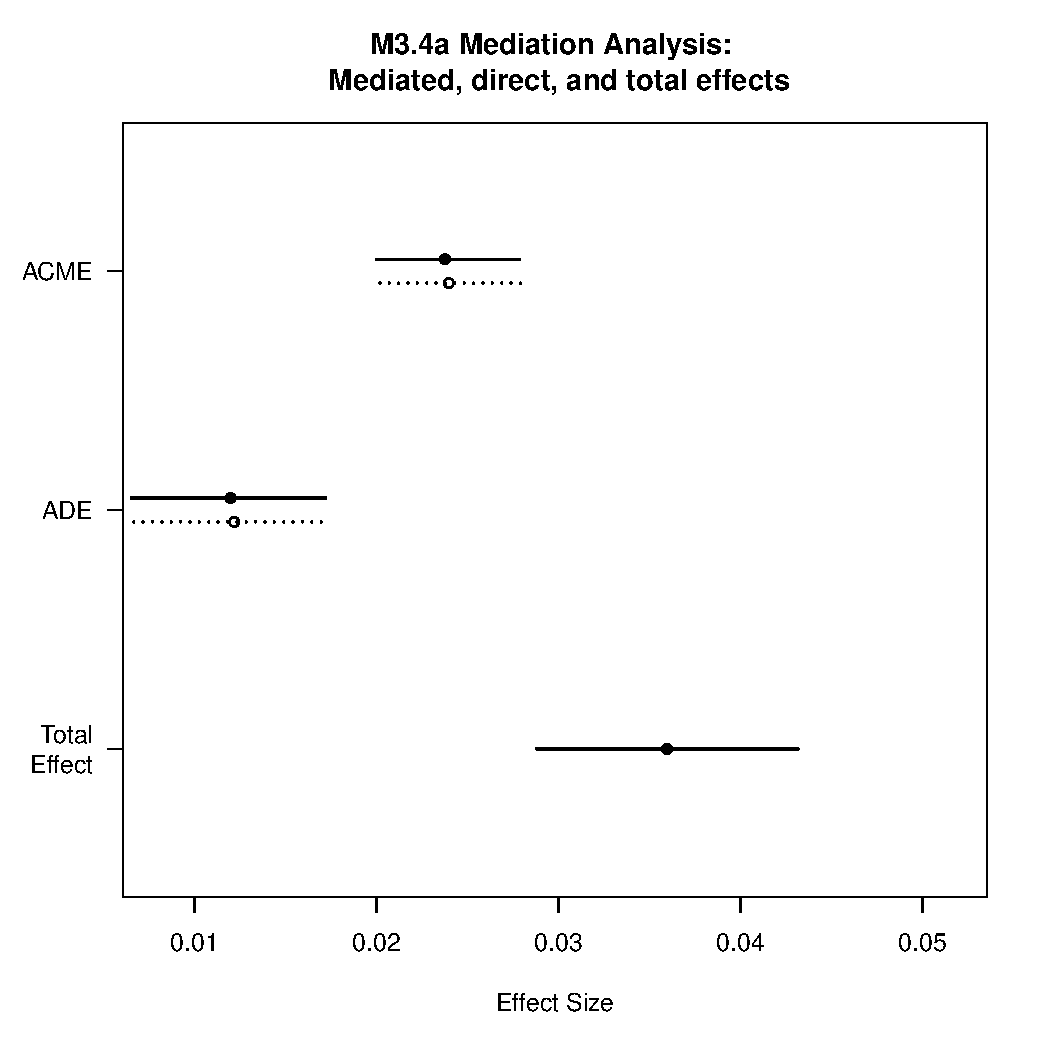
\includegraphics[width =\columnwidth]{images/MLM34aMediationAnalysis.pdf}
%  \caption{M3.4a Mediation Analysis}
%  \label{fig:MLM34aMediationAnalysis}
%\end{figure}


\subsubsection{Discussion of overall Tournament results}
